%%%%%%%%%%%%%%%%%%%%%%%%%%%%%%%%%%%%%%%%%%%%%%%%%%%%%%%%%%%%%%%%%%%%%%
% LaTeX Example: Project Report
%
% Source: http://www.howtotex.com
%
% Feel free to distribute this example, but please keep the referral
% to howtotex.com
% Date: March 2011 
% 
%%%%%%%%%%%%%%%%%%%%%%%%%%%%%%%%%%%%%%%%%%%%%%%%%%%%%%%%%%%%%%%%%%%%%%
% How to use writeLaTeX: 
%
% You edit the source code here on the left, and the preview on the
% right shows you the result within a few seconds.
%
% Bookmark this page and share the URL with your co-authors. They can
% edit at the same time!
%
% You can upload figures, bibliographies, custom classes and
% styles using the files menu.
%
% If you're new to LaTeX, the wikibook is a great place to start:
% http://en.wikibooks.org/wiki/LaTeX
%
%%%%%%%%%%%%%%%%%%%%%%%%%%%%%%%%%%%%%%%%%%%%%%%%%%%%%%%%%%%%%%%%%%%%%%
% Edit the title below to update the display in My Documents
%\title{Project Report}
%
%%% Preamble
\documentclass[paper=a4, fontsize=11pt]{scrartcl}
    \usepackage[T1]{fontenc}
    \usepackage{fourier}
    
    \usepackage[english]{babel}															% English language/hyphenation
    \usepackage[protrusion=true,expansion=true]{microtype}	
    \usepackage{amsmath,amsfonts,amsthm} % Math packages
    \usepackage[pdftex]{graphicx}	
    \usepackage{url}
    
    
    %%% Custom sectioning
    \usepackage{sectsty}
    \allsectionsfont{\centering \normalfont\scshape}
    
    
    %%% Custom headers/footers (fancyhdr package)
    \usepackage{fancyhdr}
    \pagestyle{fancyplain}
    \fancyhead{}											% No page header
    \fancyfoot[L]{}											% Empty 
    \fancyfoot[C]{}											% Empty
    \fancyfoot[R]{\thepage}									% Pagenumbering
    \renewcommand{\headrulewidth}{0pt}			% Remove header underlines
    \renewcommand{\footrulewidth}{0pt}				% Remove footer underlines
    \setlength{\headheight}{13.6pt}
    
    
    %%% Equation and float numbering
    \numberwithin{equation}{section}		% Equationnumbering: section.eq#
    \numberwithin{figure}{section}			% Figurenumbering: section.fig#
    \numberwithin{table}{section}				% Tablenumbering: section.tab#
    
    
    %%% Maketitle metadata
    \newcommand{\horrule}[1]{\rule{\linewidth}{#1}} 	% Horizontal rule
    
    \title{
            %\vspace{-1in} 	
            \usefont{OT1}{bch}{b}{n}
            \horrule{0.5pt} \\[0.4cm]
            \huge ICS 674 Mini Project: Random Genetic String Matcher (A Slight Biological Approach)\\
            \horrule{2pt} \\[0.5cm]
    }
    \author{
            \normalfont 								\normalsize
            Anson Yu \\[-3pt]		                    \normalsize
            \today
    }
    \date{}
    
    
    %%% Begin document
    \begin{document}
    \maketitle
    \section{Introduction}
    As an introduction to genetic algorithms, I made basic genetic string matcher where the main idea is that
    given a random initial population of strings, the algorithm will generate a fixed population of random strings.
    The algorithm has a target string that one of the random strings must reach or else the application will not 
    terminate, this may cause issues in performance depending on the run.  The mutation function is random in the sense
    that there is a 50/50 chance that when the function is mutating, there is also a chance that nothing happens or a 
    mutation does occur.  The same can be said about the crossover function as well where there is a 50/50 chance a 
    crossover may occur.  The competition in the algorithm is basic in that the competition is for the population
    to compete with it's next nearing neighbor.  The main factors that change the rate and time is the length of strings, 
    the size of the population, and the chance for mutations and recombinations to occur.
    \begin{align} 
        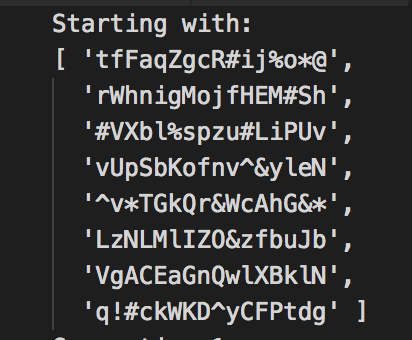
\includegraphics[scale=0.6]{randomStringsPopulation}				
    \end{align}
   The above is an example of the random strings from which my initial population came from before evolution. From these 
   strings, I create a an N amount population that mutates into a new generation that works to get closer and closer to
   the target string that I set it too.

    \subsection{Tools Used}
    The tools I used for this project was Node Javascript and a node package called ``geneticalgorithm'' which provided
    a slight template for the algorithm that may be written.  The developer has the following responsibilties when it comes to 
    actual implementation of the algorithm:

    \begin{itemize}
        \item Implementing the fitness function
        \item Implementing the mutation function
        \item Implementing the crossover function
        \item Implementing the phenotype(s) to evolve
        \item Implementing how you get the metrics for scores
        \item Implementing the control over the output of the algorithm
        \item (Optionally) Implementing a Competition Function
    \end{itemize}

    \section{Details of Project}
    In this section, I will explain the details of the project such as defining the search space, objective function,
    variation operators, and selection function.  Algorithm-wise there is alot based on randomness which determines
    how the generations may occur therefore no two runs of the evolution are exactly the same, however the amount of 
    generations is roughly in the same ballpark of $+/-$ 50 generations.  However adding randomness and probability 
    into mutations and crossover chances do indeed add even more variations into the mix and the amount of generation
    may grow exponentially which does cause performance issues from time to time.


    \subsection{Search Space}
    The search space for the algorithm varied depending on the length of the target string that I decided I want the 
    program to converge on.  The possible pool of characters is shown below and there are a total of 60 possible characters
    to choose from for the string, therefore depending on the lenghth of the string, we would have search space of size
    $60^{targetStringLength}$.
    \begin{align} 
        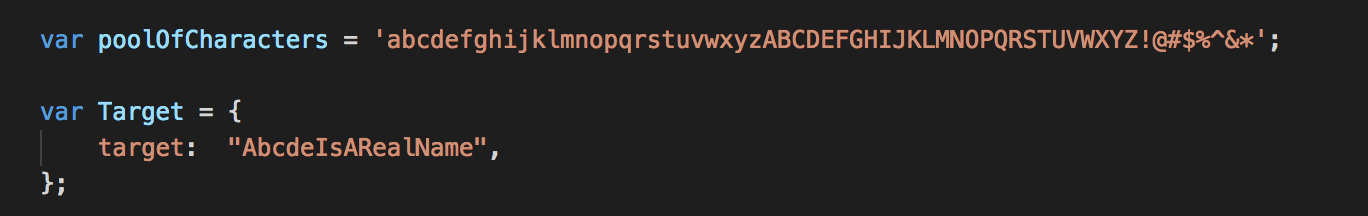
\includegraphics[scale=0.6]{SearchSpace}				
    \end{align}

    Based on the example above, the target string ``AbcdeIsARealName'' is of length $16$ and therefore the search space
    is $60^{16}$ or the size of roughly $2.82\times10^{28}$.
    
    \subsection{Objective/Fitness Function}
    The Objective function is a simple function that compares the inputted string and compares character for character
    to the target string.  The objective function then inputs a plus one score if the same index of each string is the 
    same character.  In the case the characters the two compared indexes are not the same, we use ASCII code values and increment
    the fitness by the code value divided by 60 to represent that the index was getting warmer and warmer to the target string.
    \begin{align} 
        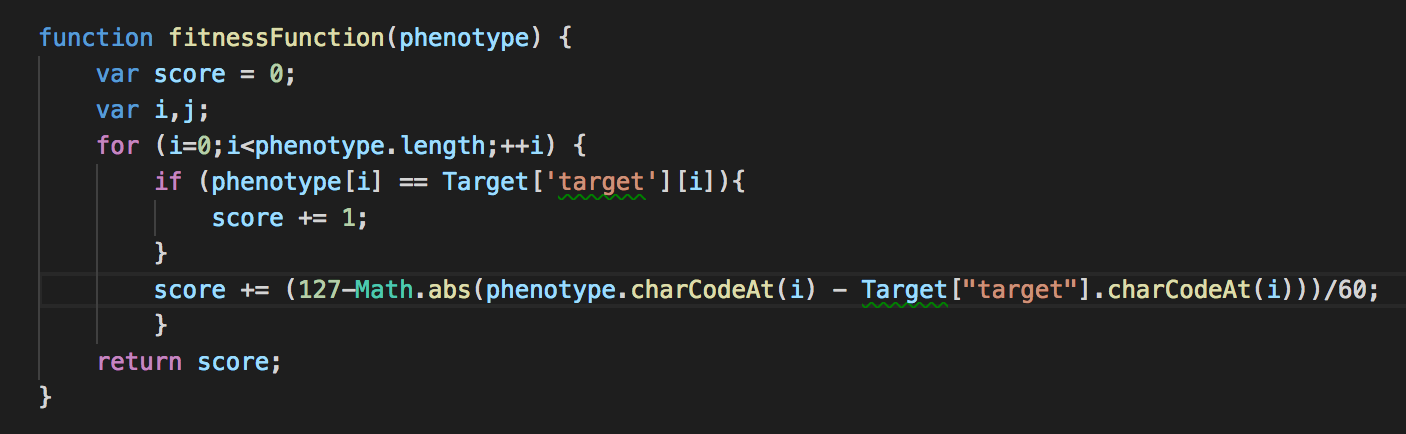
\includegraphics[scale=0.6]{ObjectiveFunction}				
    \end{align}

    \subsection{Variation Functions}
    The variation function we have are a crossover function and a mutation function.  Each of them add a random
    chance probability that the occurance of a silent mutation and the actual may occur.  This will be further 
    elaborated on when the selection functions are explained in the next section of this paper.

    \subsubsection{Mutation Function}
    The mutation function is simple in that it will first have a 50\% chance of the mutation actually surfacing,
    hence a possible silent mutation.  When the mutation does actually occur, what it will do is replace a random
    character in the string with a character from the gene pool  and return the mutant string.  When the mutation 
    does not occur, the function will just return initial string.
    \begin{align} 
        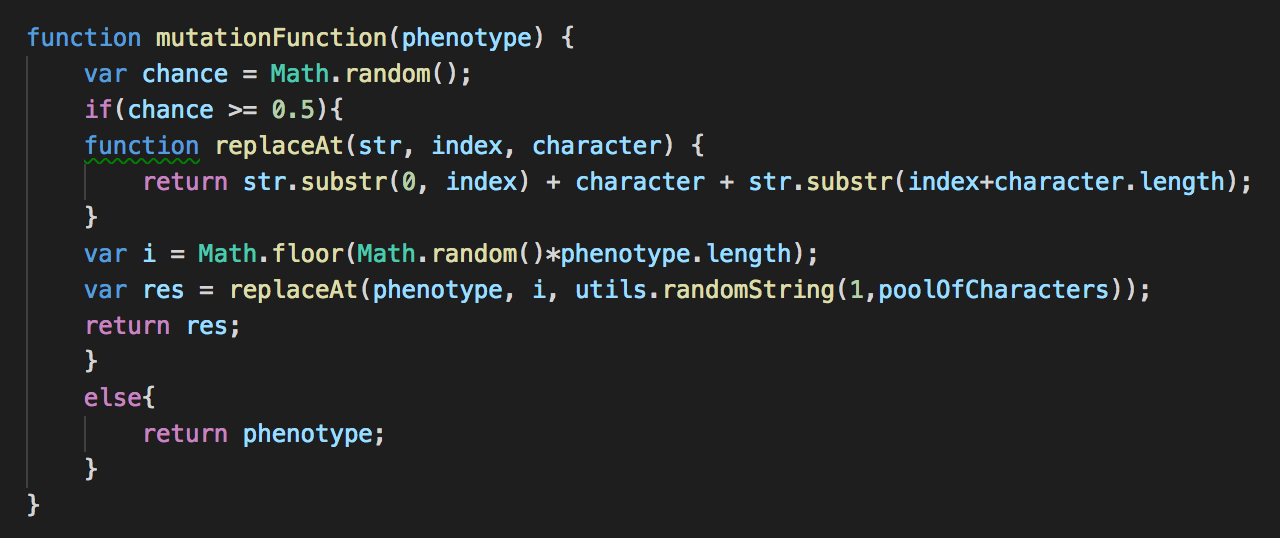
\includegraphics[scale=0.5]{MutationFunction}				
    \end{align}

    \subsubsection{Crossover Function}
    The crossover function is straightfoward with the added probability that even if there is a chance of crossover
    due to proximity, the crossover itself may not occur.  On the chance that a crossover occur's,  the function 
    will generate two random length/index values that will serve to decide the substrings of a random 
    length in the same indices that the function will swap to produce two new strings.  This serves a mimic of 
    two-point crossover.
    \begin{align} 
        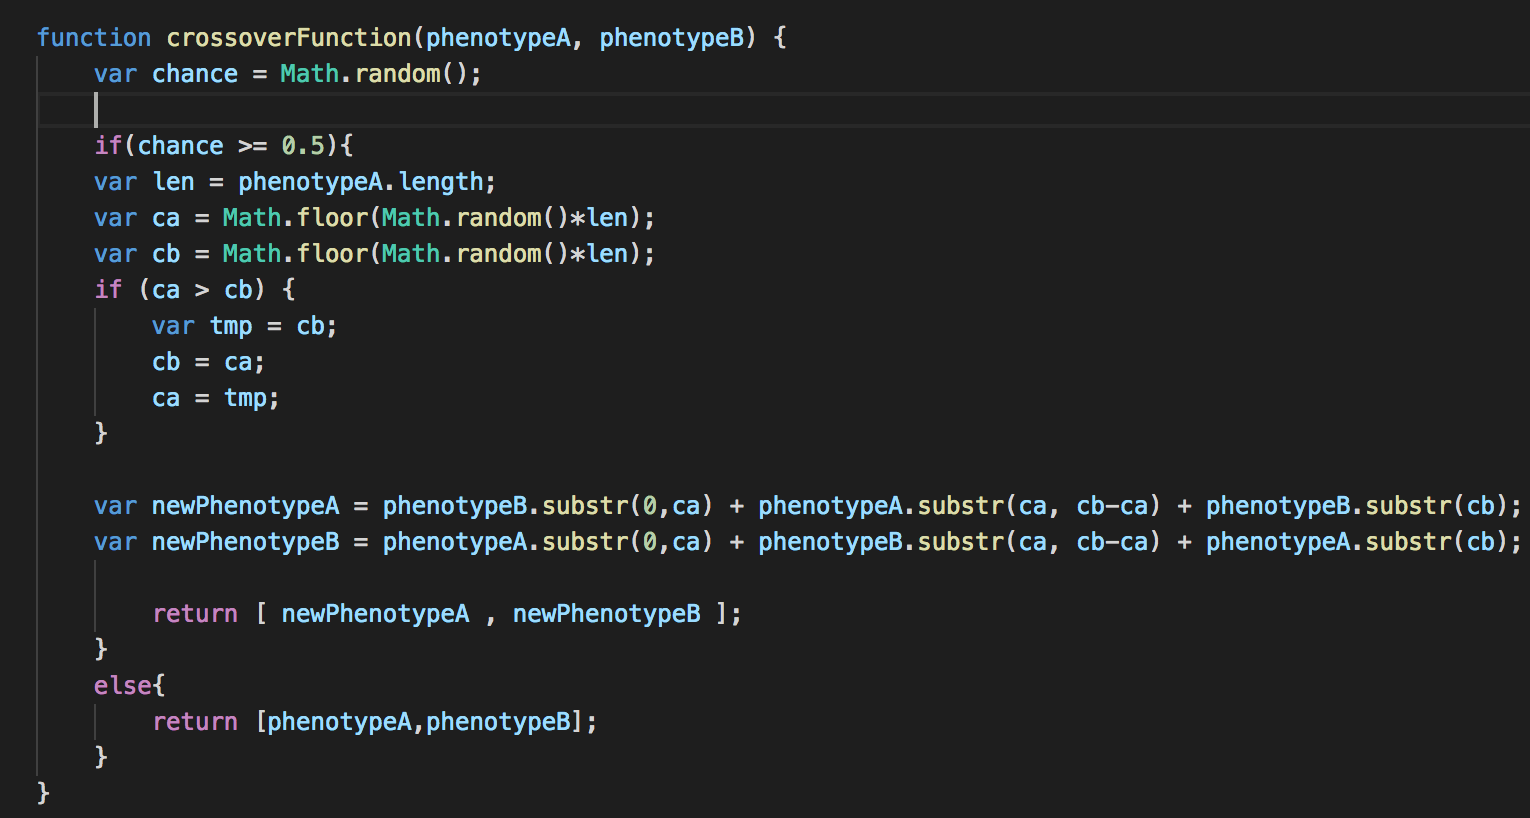
\includegraphics[scale=0.45]{CrossoverFunction}				
    \end{align}
    \subsection{Selection Operator}
    The selection operators are straightforward competition algorithms and was done in two different manners.
    The underlying mechanic however is that when two neighboring strings  are compared, the one with the larger fitness
    score is the one who wins.  To explain in more detail, lets label the two competing strings as original and neighbor,  
    if the winner is the neighbor, they will take the spot of the original in the next generation.  However if the 
    original wins, they undergo a chance for either mutation or crossover to enhance it even further in the next generation.
    \begin{align} 
        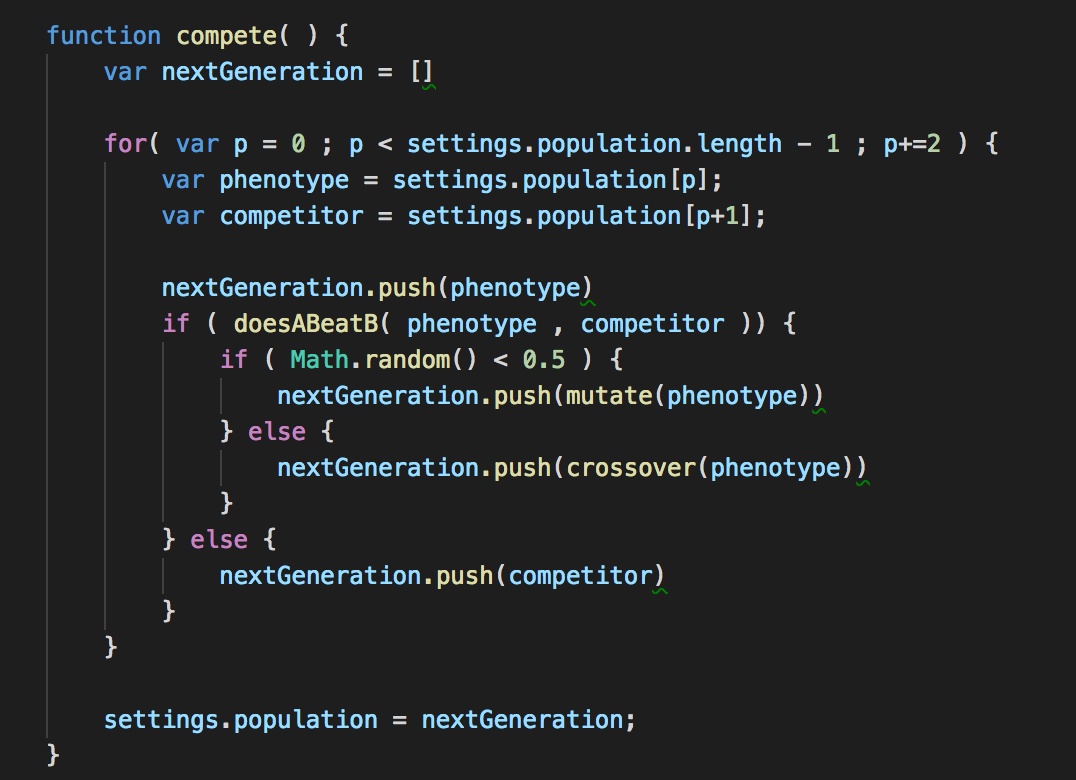
\includegraphics[scale=0.44]{CompetitionAlgorithm}				
    \end{align}

    \subsubsection{Disease and No Disease}
    Below we see the simple competition where we can rely on no outside factors detering the string from evolving and the 
    only threat they have is each other.  Hence we can see the underlying idea of just returning the function with the 
    better fitness score.
    \begin{align} 
        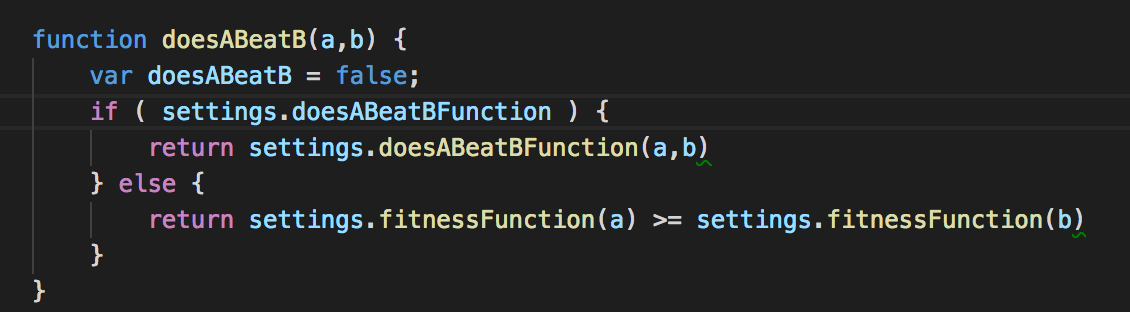
\includegraphics[scale=0.5]{SimpleCompetition}				
    \end{align}
    On this end however we find that the competition method that can be used is changed in that we now have a random 
    factor of disease can have an impact of reducing the score of the fitness of strings. From this function we can now 
    emulate the following scenarios: 
    \begin{itemize}
        \item Dominate strings have the chance of dying off and further increasing the amount of generations needed
        \item Weaker strings dominate stronger strings
        \item Both strings catch disease and only one of them survives
    \end{itemize}
    \begin{align} 
        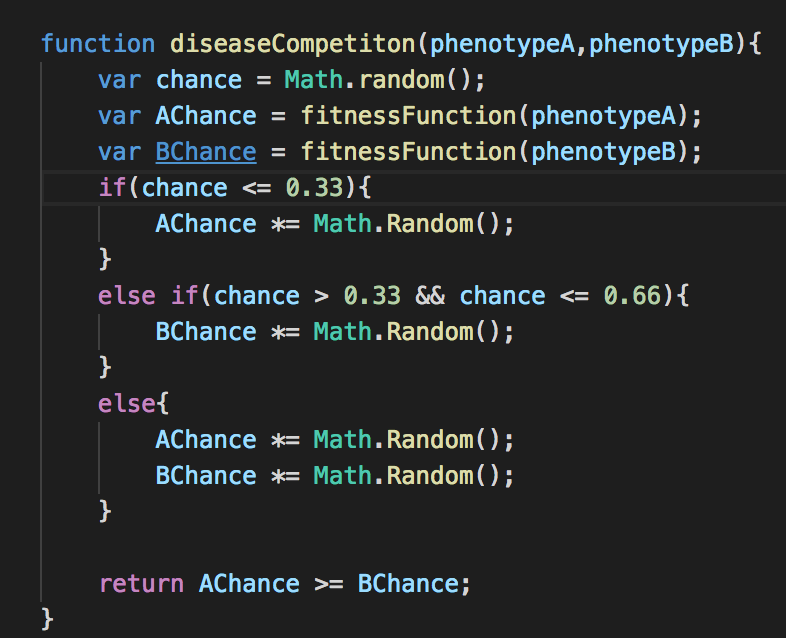
\includegraphics[scale=0.5]{DiseaseFunction}				
    \end{align}
    \subsection{Termination}
    The termination is very straightforward in that the evolution and algorithm will keep on going until a
    single string of a generated population evolves into the target string.
    \begin{align} 
        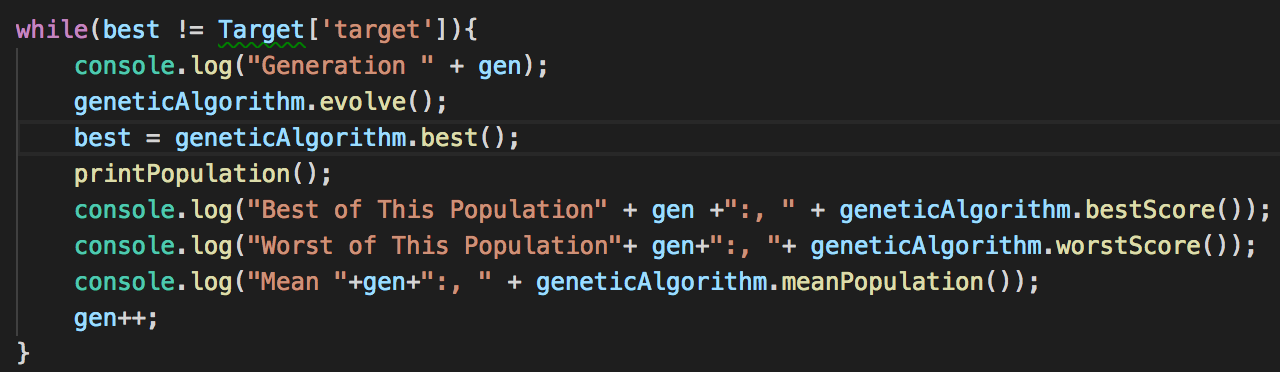
\includegraphics[scale=0.44]{Termination}				
    \end{align}

    \section{Resulting Data}
    This section covers the resulting data and will cover the trajectory of populations of two instances of 
    runs.  These two differ in that the competition/selection function are marginally different in an attempt 
    to spice up the evolution.  The end result as we see below is that trajectory path wise they share similar
    trends, but one takes more generations to reach the target string compared to the other.  The obvious behavior
    saying that the disease did stall the evolution more in some degree.

    \subsection{No Disease Data}
    \begin{align} 
        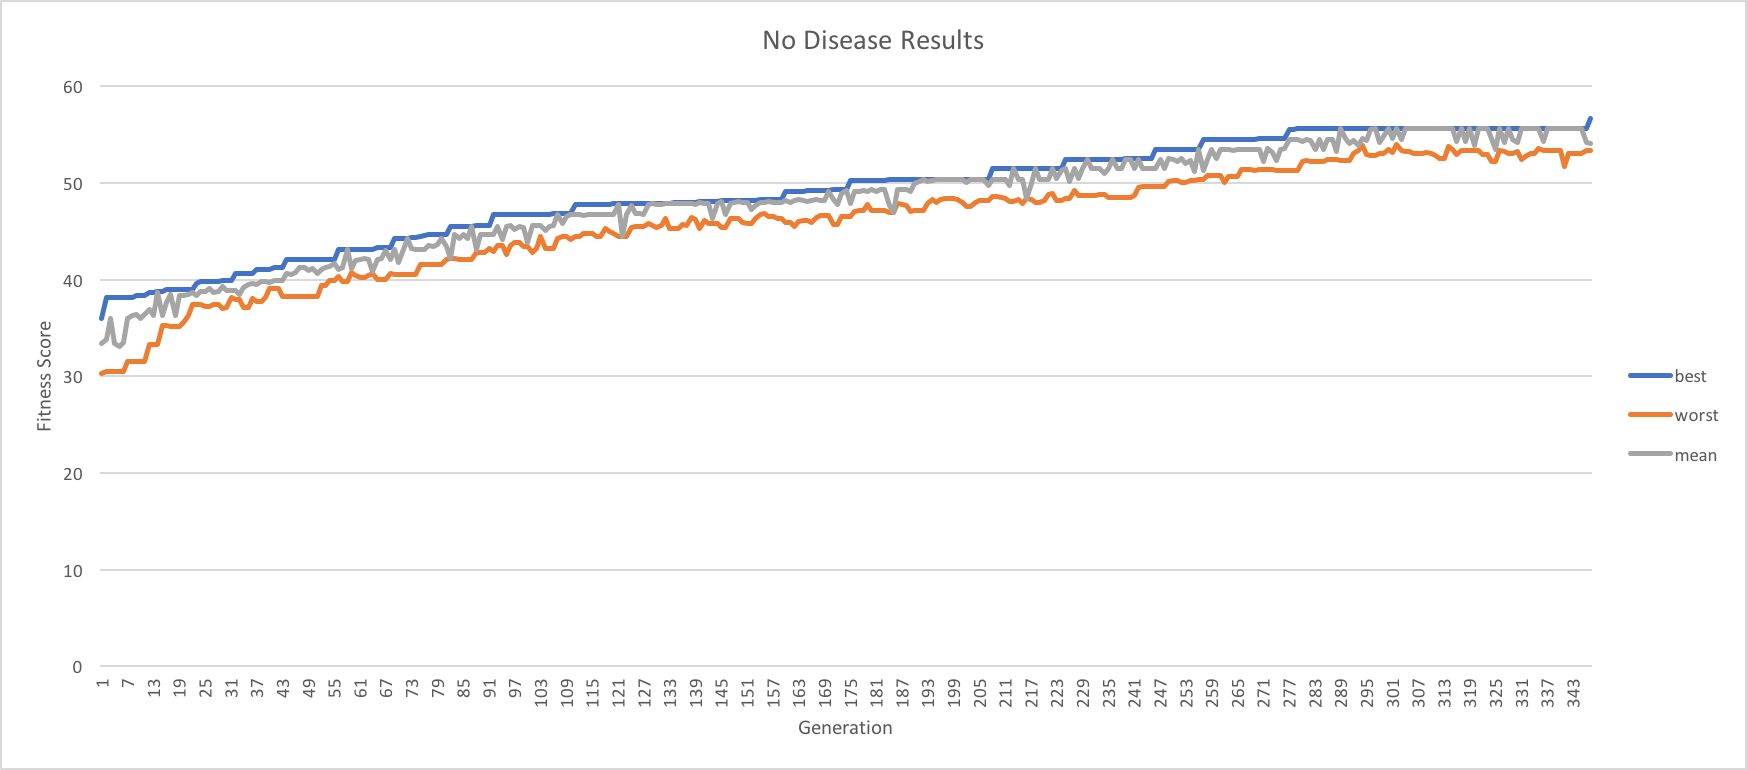
\includegraphics[scale=0.48]{NoDiseaseResults}				
    \end{align}
    \subsection{Disease Data}
    \begin{align} 
        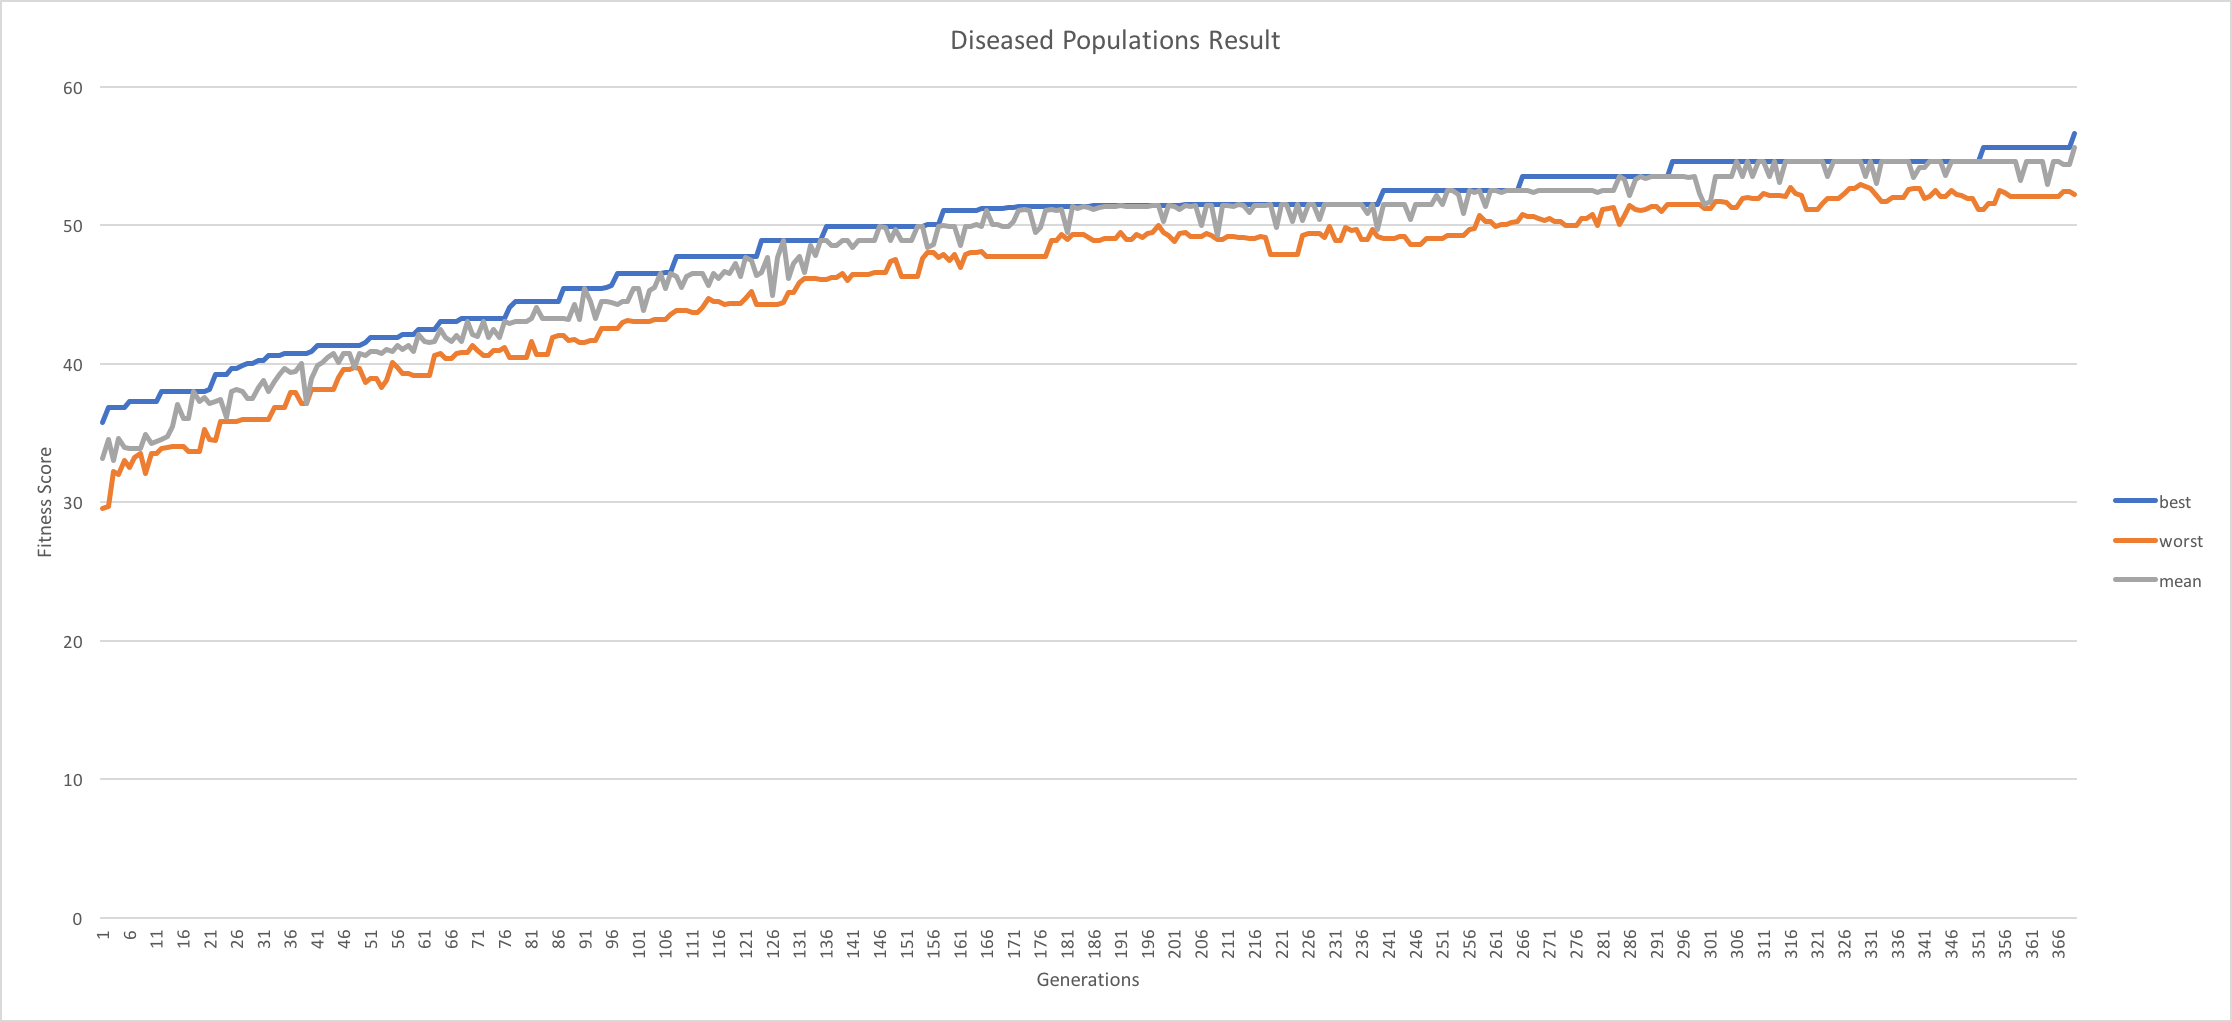
\includegraphics[scale=0.38]{DiseaseResults}				
    \end{align}

    \section{Conclusion}
    In conclusion to the study, the idea was to see how trying to replicate basic genetics behavior
    and adding pools of possibilities through additional probability would have an effect on the 
    overall growth and evolution.  While there is a strong amount of randomness,  it seeks to emulate
    from a biological standpoint what can occur when running this algorithm.  So depending on the 
    setting, throwing more and more randomness does have an obvious effect on the bounds of generation steps,
    but to reliably measure it is the challenging part.


    \end{document}